\documentclass[a4paper,11pt]{article}
\usepackage[utf8]{inputenc}
\usepackage[T3,T1]{fontenc}
\usepackage[english,ngerman]{babel}
\usepackage[noenc]{tipa}
\usepackage{tipx}
\usepackage{pifont}
\usepackage{eurosym}
\usepackage{amsmath}
\usepackage{wasysym}
\usepackage{amssymb,amsfonts,textcomp}
\usepackage{color}
\usepackage{array}
\usepackage{hhline}
\usepackage{hyperref}
\usepackage{graphicx}
\hypersetup{pdftex, colorlinks=true, linkcolor=blue, citecolor=blue, filecolor=blue, urlcolor=blue, pdftitle=, pdfauthor=, pdfsubject=, pdfkeywords=}
% Text styles
\newcommand\textstyleSourceText[1]{\texttt{#1}}
% Outline numbering
\setcounter{secnumdepth}{3}
\renewcommand\thesection{\arabic{section}}
% List styles
\newcommand\liststyleLi{%
\renewcommand\labelitemi{•}
\renewcommand\labelitemii{{\SmallCircle}}
\renewcommand\labelitemiii{{\FilledSmallSquare}}
\renewcommand\labelitemiv{•}
}
% Page layout (geometry)
\setlength\voffset{-1in}
\setlength\hoffset{-1in}
\setlength\topmargin{2cm}
\setlength\oddsidemargin{2cm}
\setlength\textheight{25.699cm}
\setlength\textwidth{16.999cm}
\setlength\footskip{0.0cm}
\setlength\headheight{0cm}
\setlength\headsep{0cm}
% Footnote rule
\setlength{\skip\footins}{0.119cm}
\renewcommand\footnoterule{\vspace*{-0.018cm}\setlength\leftskip{0pt}\setlength\rightskip{0pt plus 1fil}\noindent\textcolor{black}{\rule{0.25\columnwidth}{0.018cm}}\vspace*{0.101cm}}
% Pages styles
\makeatletter
\newcommand\ps@Standard{
  \renewcommand\@oddhead{}
  \renewcommand\@evenhead{}
  \renewcommand\@oddfoot{}
  \renewcommand\@evenfoot{}
  \renewcommand\thepage{\arabic{page}}
}
\bibliographystyle{plain}

\title{Hardwarenahe System- und Treiberprogrammierung}
%\subtitle{Parallelportcontroller MosChip MCS9815}
\author{\parbox{7cm}{Rolf Behrens und Christian Lins}}

\begin{document}
\sloppy

\maketitle
\tableofcontents
\section{Zweck des Dokumentes}
Im Rahmen der Lehrveranstaltung \textit{Hardwarenahe System- und Treiberprogrammierung} im Studiengang \textit{Verteilte und mobile Anwendungen (M.Sc)} der Hochschule Osnabrück soll in Gruppenarbeit eine Projektarbeit durchgeführt werden. Dieses Dokument dient zur Dokumention der geleisteten Arbeit und beleuchtet die gewählte Herangehensweise und die eingesetzten Technologien.

\section{Einleitung}

Eine weit verbreitete Schnittstelle in PC-Systemen zum Datenaustausch mit Peripheriegeräten stellte über Jahre hinweg die Centronics-Schnittstelle dar. Ursprünglich wurde sie bereits Ende der 1960er Jahre entwickelt. Die Druckerfirma Centronics nutze sie zunächst für die Kommunikation mit den eigenen hergestellten Druckern, im Laufe der Zeit setzten aber auch viele andere Firmen (wie IBM) auf die Schnittstelle. Obwohl Centronics die Spezifikationen offenlegte, zeigten sich oftmals in den Implementierungen anderer Hersteller kleinere Inkompatibilitäten, die sich in gewissen Details äußerten.Trotz dieser kleineren Probleme entwickelte sich die Centronics-Schnittstelle zu einem Quasi-Standard zum Ansprechen von Druckern und anderer Peripherie. Von der IEEE wurde 1994 der Standard IEEE 1284 verabschiedet, der als \textit{parallele Schnittstelle} die Centronics-Schnittstelle ablöste, aber dennoch kompatibel zum alten \textit{Centronics-Standard} blieb. 
\begin{figure}[h]
 \centering
 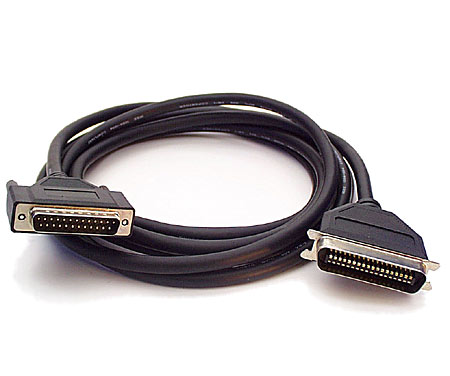
\includegraphics[scale=0.5]{./pics/IEEE1284Printercable_2007_04.jpg}
	\caption{IEEE 1284-Druckerkabel (Typ AB)} 	
\end{figure}
Der IEEE-Standard definiert die elektrischen Eigenschaften der Schnittstellen, die zu verwendenden Hardwareprotokolle und die zugehörigen Kabel. Für softwareseitige Protokolle wird auf Substandards verwiesen, die u.a. auch unabhängig von der eigentlichen Hardware agieren können. Heutzutage ist die parallele Schnittstelle (LPT) größtenteils durch modernere Schnittstellen, wie USB, ersetzt worden und erfährt nicht mehr die gleiche Bedeutung wie noch in den 1990er Jahren. 

 
\subsection{Aufgabenstellung und Projektziel}

Moderne PCs und Notebooks verzichten heutzutage bereits oft auf die parallele Schnittstelle und bieten für zusätzliche Peripheriegeräte dafür USB-Anschlüsse. Zwar sieht der ATX-Gehäusestandard noch farbliche Kennungen für LPT-Schnittstellen vor, bindend muss aber kein Hersteller diese Schnittstelle auf seinen Platinen integrieren. Um dennoch z.B. ältere Drucker in modernen Systemen verwenden zu können, bietet sich der Einsatz von PCI-Adapterkarten an, die über den PCI-Bus nach Außen hin einen Anschluss für die parallele Schnittstelle liefern. Die Implementierung eines Linux-Treibers einer solchen PCI-Adapterkarte soll Gegenstand dieser Projektarbeit sein. 

\subsection{Eingesetzte Hardware}  

Als Hardwareziel kommt eine PCI-Karte der Firma Exsys Inc (http://www.exsys.com) zum Einsatz, auf der ein Chip der Firma Moschip (http://www.moschip.com/) zum Einsatz kommt. Der dort verwendete Mikrocontroller stellt einen MCS9815-Chip dar, der die PCI zu LPT-Kommunikation übernimmt. Zwar findet sich im Linux-Kernel bereits ein Treiber für diesen Mikrokontroller, aufgrund geringer Projekteressourcen fehlt es jedoch an weiteren Alternativen. Da diese Projektarbeit eher dem lehrhaften Charakter einer studentischen Arbeit entspricht und die PCI-Karte den Projektteilnehmern bereits vorliegt, stellt die Entwicklung eines zusätzlichen Treibers für diese Karte nicht nur eine gute Übung dar, sondern ist auch gleichzeitig eine Herausforderung eine tatsächlich existierende Hardware unter dem Betriebssystem Linux zum Laufen zu bringen.  

\section{Parallelportschnittstelle}

\section{Parport-Treiber in Linux}

Da die Parallelportschnittstelle aus der Steinzeit der PC-Entwicklung stammt, ist die Unterstützung
dafür im Linux-Kernel sehr gut. 
Das \verb|parport| Subsystem besteht im Wesentlichen aus zwei Teilbereichen, einem abstrakteren Highlevel-System, das
die IEEE 1284 Kommunikation beherrscht und einem Lowlevel-System, was den Hardwarezugriff auf die einzelnen Ports
kontrolliert. Auf einem PC stellt das Modul \verb|parport_pc| den architekturspezifischen Teil bereit, das Modul parport 
den generischen Teil (vgl. \cite{net:1}).

Der hardwarespezifische Treiber registriert einen \emph{Port}\footnote{Port ist hier die logische Parallelschnittstelle, nicht zu verwechseln
mit dem I/O-Port (z.B. 0x378), der im PC für den Zugriff auf die Parallelporthardware verwendet werden kann} 
im \verb|parport| Subsystem. 
Dieses benachrichtigt alle registrierten Highlevel-Treiber (z.B. der Gerätetreiber \verb|lp| für Drucker) über den neuen Port. Der Lowlevel-Treiber stellt
Funktionen für den Zugriff auf Basisfunktionen des Ports bereit (vgl. \cite{net:1}).

Aufgabe dieser Hausarbeit ist es, einen Lowlevel-Treiber für einen speziellen Parallelport-Controller zu schreiben. Diese 
Funktionalität ist normalerweise im architekturspezifischen Modul \verb|parport_pc| integriert.

\subsection{Strukturen}

Die Dokumentation der Strukturen wurde den Quellen des Linux-Kernels entnommen 
(vgl. \cite{net:2}, Documentation/parport-lowlevel.txt).

\subsubsection{parport\_driver}

Die Struktur \verb|parport_driver| repräsentiert einen Highlevel-Parport-Treiber.

\begin{verbatim}
struct parport_driver {
    const char *name;
    void (*attach) (struct parport *);
    void (*detach) (struct parport *);
    struct parport_driver *next;
};\end{verbatim}

Die Funktionzeiger \verb|attach| und \verb|detach| muss der Treiber zur Verfügung stellen, wenn er benachrichtigt
werden will, sobald ein neuer Parallelport im System auftaucht oder einer entfernt wird (wenn z.B. der
passende Lowlevel-Treiber entfernt wird).

\subsubsection{parport}

Die Struktur \verb|parport| repräsentiert eine logische Parallelschnittstelle.

\begin{verbatim}
struct parport {
    struct parport *next; /* next parport in list */
    const char *name;     /* port's name */
    unsigned int modes;   /* bitfield of hardware modes */
    struct parport_device_info probe_info;
                          /* IEEE1284 info */
    int number;           /* parport index */
    struct parport_operations *ops;
};\end{verbatim}

Dem Bitfeld modes kann man entnehmen, welche Modi der Schnittstelle unterstützt werden (SPP, EPP).

\subsubsection{parport\_device\_info}

\begin{verbatim}
struct parport_device_info {
    parport_device_class class;
    const char *class_name;
    const char *mfr;
    const char *model;
    const char *cmdset;
    const char *description;
};\end{verbatim} 

\subsubsection{parport\_operations}

Wie auch die Struktur \verb|file_operations| bei einem Dateisystemtreiber enthält die 
Struktur \verb|parport_operations| u.a. Funktionszeiger auf die vom Treiber unterstützten
Parallelportfunktionen.

\begin{verbatim}
struct parport_operations {
    /* IBM PC-style virtual registers. */
    void (*write_data)(struct parport *, unsigned char);
    unsigned char (*read_data)(struct parport *);

    void (*write_control)(struct parport *, unsigned char);
    unsigned char (*read_control)(struct parport *);
    unsigned char (*frob_control)(struct parport *, unsigned char mask, unsigned char val);

    unsigned char (*read_status)(struct parport *);

    /* IRQs. */
    void (*enable_irq)(struct parport *);
    void (*disable_irq)(struct parport *);

    /* Data direction. */
    void (*data_forward) (struct parport *);
    void (*data_reverse) (struct parport *);

    /* For core parport code. */
    void (*init_state)(struct pardevice *, struct parport_state *);
    void (*save_state)(struct parport *, struct parport_state *);
    void (*restore_state)(struct parport *, struct parport_state *);

    /* Block read/write */
    size_t (*epp_write_data) (struct parport *port, const void *buf, size_t len, int flags);
    size_t (*epp_read_data) (struct parport *port, void *buf, size_t len, int flags);
    size_t (*epp_write_addr) (struct parport *port, const void *buf, size_t len, int flags);
    size_t (*epp_read_addr) (struct parport *port, void *buf, size_t len, int flags);

    size_t (*ecp_write_data) (struct parport *port, const void *buf, size_t len, int flags);
    size_t (*ecp_read_data) (struct parport *port, void *buf, size_t len, int flags);
    size_t (*ecp_write_addr) (struct parport *port, const void *buf, size_t len, int flags);

    size_t (*compat_write_data) (struct parport *port, const void *buf, size_t len, int flags);
    size_t (*nibble_read_data) (struct parport *port, void *buf, size_t len, int flags);
    size_t (*byte_read_data) (struct parport *port, void *buf, size_t len, int flags);
    struct module *owner;
};\end{verbatim} 

Die einzelnen Funktionen werden in den folgenden Abschnitten erläutert.

\subsection{Funktionen}

Die Dokumentation der Funktionen wurde den Quellen des Linux-Kernels entnommen 
(vgl. \cite{net:2}, Documentation/parport-lowlevel.txt). Die meisten der angegebenen Funktionen
sollte ein Lowlevel-Treiber bereitstellen.

\subsubsection{SPP Port Funktionen}

\paragraph{write\_data}

\begin{verbatim}
void (*write_data) (struct parport *port, unsigned char d);
\end{verbatim}

Schreibt d in das Datenregister des angegebenen Ports.

\paragraph{read\_data}

\begin{verbatim}
unsigned char (*read_data) (struct parport *port);
\end{verbatim}

Liest das Datenregister des angegebenen Ports und gibt den Inhalt zurück.

\paragraph{read\_status}

\begin{verbatim}
unsigned char (*read_status) (struct parport *port);
\end{verbatim}

Liest das Statusregister des angegebenen Ports und gibt den Inhalt zurück.

\paragraph{read\_control}

\begin{verbatim}
unsigned char (*read_control) (struct parport *port);
\end{verbatim}

Gibt den Wert zurück, der zuletzt in das Controlregister geschrieben wurde. Ein Zugriff
auf die Hardware erfolgt dabei nicht.

\paragraph{write\_control}

\begin{verbatim}
void (*write_control) (struct parport *port, unsigned char s);
\end{verbatim}

Schreibt die Bitmaske s in das Controlregister des angegebenen Ports.

\paragraph{frob\_control}

\begin{verbatim}
unsigned char (*frob_control) (struct parport *port,
				unsigned char mask,
				unsigned char val);
\end{verbatim}

TODO: Vermutlich muss der Treiber das nicht implementieren. Weglassen?

This is equivalent to reading from the control register, masking out
the bits in mask, exclusive-or'ing with the bits in val, and writing
the result to the control register.

As some ports don't allow reads from the control port, a software copy
of its contents is maintained, so frob\_control is in fact only one
port access.

\paragraph{enable\_irq}

\begin{verbatim}
void (*enable_irq) (struct parport *port)
\end{verbatim}

Weist die Hardware an, in Zukunft Interrupts zu erzeugen.

\paragraph{disable\_irq}

\begin{verbatim}
void (*data_forward) (struct parport *port)
\end{verbatim}

Deaktiviert die Interrupts auf der Hardware.

\paragraph{data\_forward}

\begin{verbatim}
void (*data_forward) (struct parport *port)
\end{verbatim}

Aktiviert die Treiber des Datenports.

\paragraph{data\_reverse}

\begin{verbatim}
void (*data_reverse) (struct parport *port)
\end{verbatim}

Places the data bus in a high impedance state, if port->modes has the
PARPORT\_MODE\_TRISTATE bit set.

Blubb?

\subsubsection{EPP Port Funktionen}

\paragraph{epp\_write\_data}

\paragraph{epp\_read\_data}

\paragraph{epp\_write\_addr}

\paragraph{epp\_read\_addr}

\subsubsection{ECP und andere Portfunktionen}

\paragraph{ecp\_write\_data}

\paragraph{ecp\_read\_data}

\paragraph{ecp\_write\_addr}

\paragraph{nibble\_read\_data}

\begin{verbatim}
size_t (*nibble_read_data) (struct parport *port, void *buf, size_t len, int flags);
\end{verbatim}

Liest einen Datenblock in Nibble-Mode.

\paragraph{byte\_read\_data}

\begin{verbatim}
size_t (*byte_read_data) (struct parport *port, void *buf, size_t len, int flags)
\end{verbatim}

Liest einen Datenblock in Byte-Mode.

\paragraph{compat\_write\_data}

\begin{verbatim}
size_t (*compat_write_data) (struct parport *port, const void *buf, size_t len, int flags)
\end{verbatim}

Schreibt einen Datenblock im Kompatibilitätsmodus.

\subsection{Globale Funktionen den parport Subsystems}

Die globalen Funktionen des parport Subsystems können sowohl von den Lowlevel- als auch
Highlevel-Treibern verwendet werden.

\subsubsection{Funktionen für Lowlevel-Treiber}

\paragraph{parport\_register\_port}
\begin{verbatim}
struct parport *parport_register_port(unsigned long base, int irq, int dma, 
                                      struct parport_operations *ops)
\end{verbatim}

Sobald ein Lowlevel-Treiber einen Parallelport detektiert und diesen den Highlevel-Treibern zur
Verfügung stellen will, macht er den Port über diese Methode dem System bekannt.

Die Struktur ops darf nicht freigegeben werden, bevor nicht parport\_remove\_port für den
angegebenen Port aufgerufen wurde.

Gerätetreiber sollten danach mit parport\_announce\_port über den neuen Parallelport informiert
werden.

\paragraph{parport\_remove\_port}
\begin{verbatim}
void parport_remove_port(struct parport *port)
\end{verbatim}

Entfernt einen Parallelport aus dem System. Alle registrierten Gerätetreiber werden durch den
Aufruf ihrer jeweiligen detach Funktionen über die Entfernung des Ports informiert.

\paragraph{parport\_announce\_port}
\begin{verbatim}
void parport_announce_port (struct parport *port)
\end{verbatim}

Macht einen registrierten Parallelport bei den Gerätetreibern bekannt, in dem die jeweiligen
attach Funktionen der Gerätetreiber aufgerufen werden.

\subsubsection{Funktionen für Highlevel-Treiber}

\paragraph{parport\_register\_driver}

\begin{verbatim}
int parport_register_driver (struct parport_driver *driver);
\end{verbatim}

Damit ein Treiber über neue Parallelschnittstellen des Systems informiert wird, muss er
sich mit dieser Methode im Kernel registrieren. Nach der Registrierung wird der Treiber
sofort über alle bereits detektierten Parallelschnittstellen informiert (attach Funktion)
und über jede, die in Zukunft von einem Lowlevel-Treiber bereitgestellt oder entfernt wird.

\paragraph{parport\_unregister\_driver}

\begin{verbatim}
void parport_unregister_driver (struct parport_driver *driver);
\end{verbatim}

Nach Aufruf dieser Funktion wird der angegebene Treiber nicht mehr über die Registrierung
und Deregistrierung von Parports informiert. Die bereits registrierten Geräte werden \emph{nicht}
automatisch deregistriert.

% \paragraph{parport\_enumerate}
% Lassen wir weg, da die Funktion deprecated ist.

\paragraph{parport\_register\_device}

\begin{verbatim}
typedef int (*preempt_func) (void *handle);
typedef void (*wakeup_func) (void *handle);
typedef int (*irq_func) (int irq, void *handle, struct pt_regs *);

struct pardevice *parport_register_device(struct parport *port,
                                          const char *name,
                                          preempt_func preempt,
                                          wakeup_func wakeup,
                                          irq_func irq,
                                          int flags,
                                          void *handle);
\end{verbatim}

Diese Funktion wird verwendet um einen Gerätetreiber, der den angegebenen Parallelport verwenden will,
im parport System zu registrieren. Der gewählte Gerätename ('name') muss während der Lebenszeit des
Geräts eindeutig sein. 
Die über preempt spezifizierte Funktion wird aufgerufen, wenn ein anderer Treiber den Port verwenden
möchte (es können mehrere Geräte eine Parallelschnittstelle verwenden).
Die wakeup Funktion wird aufgerufen, sobald der Parallelport von einem anderen Treiber wieder
freigegeben wurde. Die Funktion irq wird aufgerufen, wenn am angegebenen Parallelport ein Interrupt
auftritt.

\paragraph{parport\_unregister\_device}

\begin{verbatim}
void parport_unregister_device (struct pardevice *dev)
\end{verbatim}

Deregistriert das angegebene Gerät ('dev').

\paragraph{parport\_claim und parport\_claim\_or\_block}

\begin{verbatim}
int parport_claim (struct pardevice *dev)
int parport_claim_or_block (struct pardevice *dev)
\end{verbatim}

\paragraph{parport\_release}

\begin{verbatim}
void parport_release (struct pardevice *dev)
\end{verbatim}

\paragraph{parport\_yield und parport\_yield\_blocking}

\begin{verbatim}
int parport_yield (struct pardevice *dev)
int parport_yield_blocking (struct pardevice *dev);
\end{verbatim}

\paragraph{parport\_wait\_peripheral}
\begin{verbatim}
int parport_wait_peripheral (struct parport *port,
			     unsigned char mask,
			     unsigned char val);
\end{verbatim}


\paragraph{parport\_poll\_peripheral}

\begin{verbatim}
int parport_poll_peripheral (struct parport *port,
			     unsigned char mask,
			     unsigned char val,
			     int usec);
\end{verbatim}


\paragraph{parport\_wait\_event}
\begin{verbatim}
int parport_wait_event (struct parport *port, signed long timeout)
\end{verbatim}


\paragraph{parport\_negotiate}
\begin{verbatim}
int parport_negotiate (struct parport *, int mode)
\end{verbatim}

\paragraph{parport\_read}
\begin{verbatim}
ssize_t parport_read (struct parport *, void *buf, size_t len)
\end{verbatim}

\paragraph{parport\_write}
\begin{verbatim}
ssize_t parport_write (struct parport *, const void *buf, size_t len)
\end{verbatim}


\paragraph{parport\_open}
\begin{verbatim}
struct pardevice *parport_open (int devnum, const char *name,
				int (*pf) (void *),
				void (*kf) (void *),
				void (*irqf) (int, void *,
				struct pt_regs *),
				int flags, void *handle)
\end{verbatim}


\paragraph{parport\_close}
\begin{verbatim}
void parport_close (struct pardevice *dev)
\end{verbatim}


\paragraph{parport\_device\_id}
\begin{verbatim}
ssize_t parport_device_id (int devnum, char *buffer, size_t len)
\end{verbatim}


\paragraph{parport\_device\_coords}
\begin{verbatim}
int parport_device_coords (int devnum, int *parport, int *mux, int *daisy)
\end{verbatim}

\paragraph{parport\_find\_class}
\begin{verbatim}
typedef enum {
	PARPORT_CLASS_LEGACY = 0,       /* Non-IEEE1284 device */
	PARPORT_CLASS_PRINTER,
	PARPORT_CLASS_MODEM,
	PARPORT_CLASS_NET,
	PARPORT_CLASS_HDC,              /* Hard disk controller */
	PARPORT_CLASS_PCMCIA,
	PARPORT_CLASS_MEDIA,            /* Multimedia device */
	PARPORT_CLASS_FDC,              /* Floppy disk controller */
	PARPORT_CLASS_PORTS,
	PARPORT_CLASS_SCANNER,
	PARPORT_CLASS_DIGCAM,
	PARPORT_CLASS_OTHER,            /* Anything else */
	PARPORT_CLASS_UNSPEC,           /* No CLS field in ID */
	PARPORT_CLASS_SCSIADAPTER
} parport_device_class;

int parport_find_class (parport_device_class cls, int from);
\end{verbatim}


\paragraph{parport\_find\_device}
\begin{verbatim}
int parport_find_device (const char *mfg, const char *mdl, int from)
\end{verbatim}


\paragraph{parport\_set\_timeout}
\begin{verbatim}
long parport_set_timeout (struct pardevice *dev, long inactivity)
\end{verbatim}


\section{Der MosChip MCS9815 Controller}

Der MCS9815 ist ein Parallelport Controller Chip der Firma MosChip. Er kann
zwei Parallelports über das PCI Interface an das System anbinden und unterstützt alle
aktuellen Modi (SPP, PS2, EPP, ECP) der Parallelschnittstelle.

\begin{figure}[h]
 \centering
 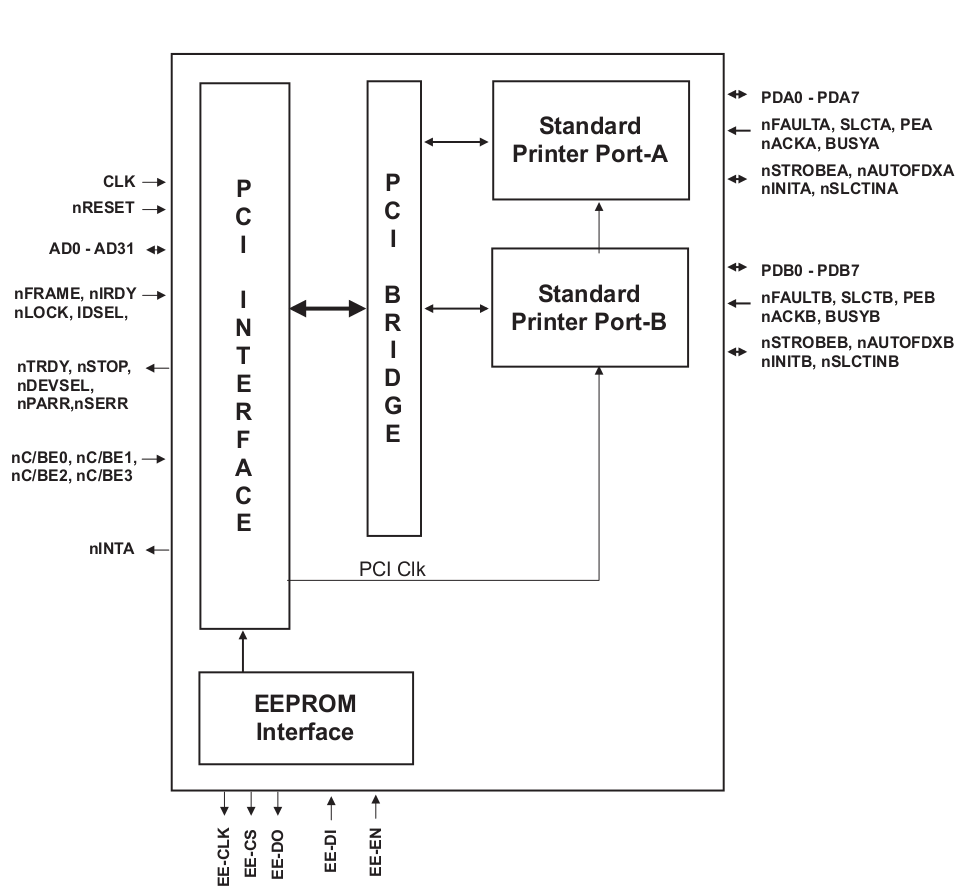
\includegraphics[bb=0 0 724 671,scale=0.5]{./pics/mcs9815_block_diagram.png}
 % mcs9815_block_diagram.png: 965x895 pixel, 96dpi, 25.53x23.68 cm, bb=0 0 724 671
\end{figure}


\bibliography{literatur}


\end{document}